\documentclass[noinfoline]{imsart}

\usepackage{Sweave}

\usepackage[english]{babel}
%\usepackage[latin1]{inputenc}
%\usepackage[T1]{fontenc}
%\usepackage{float}
\usepackage{graphicx}
\usepackage{amsmath}
\usepackage{amsfonts}
\usepackage{amssymb}    
\usepackage{amsthm}
\usepackage{url}
\usepackage{a4wide}

% fonts lisibles en ligne
\usepackage{helvet}
\renewcommand{\familydefault}{\sfdefault}
\parindent=0mm

%\usepackage{stmaryrd}
%\usepackage{url}
%\usepackage{epsfig}
%\usepackage{natbib}
\usepackage{color}
\def\cov{\mbox{cov}}
\def\var{\mbox{Var}}
\def\corr{\mbox{corr}}
\def\DKhi{\mathrm{DKhi}}
\def\EDKhi{\mathrm{EDKhi}}
\def\Tr{\mathrm{Tr}}
\def\X{{\tt X}}
\def\D{{\tt dmax}}

% maths-Ensembles

\def\1{{\mathbf 1}}
\def\N{{\mathbb{N}}}
\def\Z{{\mathbb{Z}}}
\def\Q{{\mathbb{Q}}}
\def\R{{\mathbb{R}}}
\def\C{{\mathbb{C}}}
\def\E{{\mathbb{E}}}
\def\P{{\mathbb{P}}}
\def\L{{\mathbb{L}}}

%Nouvelles commandes

\newcommand{\eref}[1]{(\ref{#1})}
\newcommand{\pa}[1]{\left({#1}\right)}
\newcommand{\croa}[1]{\Big[{#1}\Big]}
\newcommand{\cro}[1]{\left[{#1}\right]}
\newcommand{\ab}[1]{\left|{#1}\right|}
\newcommand{\aca}[1]{\Bigg\{{#1}\Bigg\}}
\newcommand{\ac}[1]{\left\{{#1}\right\}}
\newcommand{\norm}[1]{\left\|{#1}\right\|}

%\psfigdriver{dvips}
%\usepackage{mathrsfs}

%\parindent=0mm


%\usepackage{geometry}
%\newfloat{Figure}{H}{lof}
%\newfloat{Table}{Hptb}{lot} 

\newtheorem{thrm}{Theorem}[section]
\newtheorem{prte}[thrm]{Proposition}
\newtheorem{lemma}[thrm]{Lemma}
\newtheorem{cor}[thrm]{Corollary}
\newtheorem{defi}[thrm]{Definition}
\newtheorem{remark}[thrm]{Remark}
\newtheorem{ex}[thrm]{Example}
\newtheorem{algo}[thrm]{Algorithm}
\newenvironment{Proof}{~\newline\textbf{Proof:}}{\begin{flushright} $\blacksquare$ \end{flushright}~\\}


\newcommand{\degr}{\mathrm{deg}} 
\newcommand{\pen}{\mathrm{pen}}
\newcommand{\LA}{\mathrm{LA}}
\newcommand{\EW}{\mathrm{EW}}
\newcommand{\QE}{\mathrm{QE}}
\newcommand{\CO}{\mathrm{C0}}
\newcommand{\nei}{\mathrm{ne}}
\newcommand{\crit}{\mathrm{Crit}}
\newcommand{\supp}{\mathrm{supp}}
\newcommand{\MSEP}{\mathrm{MSEP}}
%\newcommand{\X}{{\bf X}}

% NOUVELLES COMMANDES
\def\B{{\mathbb{B}}}
\def\G{\mathcal{G}}
\def\thetat{\tilde \theta}
\def\eps{\boldsymbol{\epsilon}}


% Profondeur table of contents
\setcounter{tocdepth}{2}     % Dans la table des matieres
\setcounter{secnumdepth}{3}  % Avec un numero.


\begin{document}
\begin{frontmatter}
\title{GGMselect:  R package for estimating Gaussian graphical models}

\runtitle{ GGMselect}
%\VignetteIndexEntry{GGMselect:  Introduction and User Guide}
\begin{aug}
\author{\fnms{Annie} \snm{Bouvier}\ead[label=e1]{Annie.Bouvier@inra.fr}},
\author{\fnms{Christophe} \snm{Giraud}\ead[label=e2]{Christophe.Giraud@polytechnique.edu}},
\author{\fnms{Sylvie} \snm{Huet}\ead[label=e3]{Sylvie.Huet@inra.fr}},
\and	
\author{\fnms{Nicolas} \snm{Verzelen}\ead[label=e4]{nicolas.verzelen@math.u-psud.fr}}
\address{INRA, MaIAGE, 78352 Jouy-en-Josas Cedex, FRANCE\\ \printead{e1}}
\address{Ecole Polytechnique, CMAP, UMR 7641\\ Route de Saclay 
91128 Palaiseau Cedex, FRANCE  \\ \printead{e2}}
\address{INRA, MaIAGE, 78352 Jouy-en-Josas Cedex, FRANCE\\ \printead{e3}}
\address{Universit\'e Paris Sud, Laboratoire de Math\'ematiques, UMR 8628\\ Orsay Cedex F-91405\\ \printead{e4}}
\runauthor{Bouvier, Giraud,  Huet, and  Verzelen }
\end{aug}



%\received{\smonth{2} \syear{2011}}
\end{frontmatter}


\maketitle


\centerline{{Contact:} {\tt Sylvie.Huet@inra.fr}}
\medskip

\tableofcontents

\section{Introduction}


 Biotechnological developments in proteomics or transcriptomics enable to produce a
huge amount of  data. One of the challenges
for the statistician  is to infer from these data the regulation network of a
family of  genes (or proteins). Gaussian graphical models are promising probabilistic tools to achieve this challenge.

Graphical modeling is based on the conditional independence
concept: a direct relation between two variables exists if those two
variables are conditionally dependent given all the remaining
variables. 
These direct relations are represented by a graph: a node is associated to each variable and an edge is set between two nodes when they are in direct relation.
In the Gaussian setting, a direct relation between two
variables corresponds to a non-zero entry in the partial correlation
matrix, or equivalently to a non-zero entry in the inverse of the
covariance matrix. 

Let us consider  $p$ genes  that will compose the nodes of the
graph.  For each gene  we observe some random response such as  the differential
expression on microarray experiment. The $p$ nodes of the
graph are thus identified with $p$
random variables denoted by $(X_{1}, \ldots, X_{p})$ assumed to be
distributed as a multivariate Gaussian 
$\mathcal{N}(0,\Sigma)$. 
The graph $G_{\Sigma}$ of conditional dependences is defined as
follows: there exists an edge between nodes $a$ and
$b$ if and only if the variables $X_{a}$ and  $X_{b}$ are dependent
given all the remaining variables. This will be denoted 
$$a\stackrel{G_{\Sigma}}{\sim} b.$$
GGMselect \cite{GHV} is dedicated to the estimation of the graph
$G_{\Sigma}$ on the basis of a $n$-sample from
$\mathcal{N}(0,\Sigma)$. In the following, a  graph $G$ will be identified with the set of its
edges.

\medskip


GGMselect is  a two-stage procedure: 

\begin{enumerate}
 \item A family   $\widehat\G$ of candidate graphs is built using either some data-driven method or some prior knowledge on the true graph.
\item  A graph $\widehat{G}$ is
  selected among this family  $\widehat\G$ by minimizing an empirical criterion based on conditional least-squares.
\end{enumerate}

\medskip
GGMselect is specially designed to handle
the case where the sample size $n$ is smaller than the number of
variables $p$. 
Its performances  have been assessed in \cite{GHV}. 
It has been shown to be consistent even when $p$ is much larger than
$n$, 
and its risk  is controlled by a non-asymptotic oracle-like inequality. The assumptions needed to establish these results are weaker than those commonly used in the literature. In addition, numerical experiments have shown a nice behavior on simulated examples.

\medskip
\noindent{\bf Download}: \url{http://genome.jouy.inra.fr/logiciels/GGMselect/}



\medskip
\noindent{\bf Notations.} 
We set $\Gamma=\ac{1,\ldots,p}$ and for any graph $G$ with nodes
indexed by $\Gamma$, we write $d_{a}(G)$ for the degree of the node
$a$ in the graph $G$ (which is the number of edges incident to $a$)
and $\degr(G)=\max_{a\in \Gamma}d_{a}(G)$ for the degree of $G$. 
We
also write  $\|.\|_{n}$ for the Euclidean norm on $\R^n$
divided by $\sqrt n$ and for any $\beta\in\R^p$ we define
supp$(\beta)$ as the set of the labels $a\in\Gamma$ such that
$\beta_{a}\neq 0$. 


\section{Estimation procedure}


The main inputs are:\smallskip

\begin{tabular}{lp{13cm}}
 {\tt X} & A data matrix ${\X}$ of size $n\times p$. Each row corresponds to an independent observation of the vector $(X_1,\ldots, X_p)$.  We write $\X_{a}$ for the $a^{\textrm{th}}$ column of $\X$.\\
{\tt dmax} &  A vector of $p$ integers: for each $a \in
  \Gamma$,  {\tt dmax}$[a]$   is the  maximum  degree of the node $a$ within the graphs of the family $\widehat{\G}$. For each $a\in\Gamma$, $\D[a]$ must be smaller than $\min(n-3,p-1)$.\\
  % Default value is ${\tt dmax}={\tt rep(\min(3,n-3,p-1),p)}$. 
{\tt K} & A scale-free tuning parameter ${\tt K}>1$. Default value is ${\tt K}=2.5$.
\end{tabular}
\medskip


\fbox{
\begin{minipage}{0.9\textwidth}
{\bf GGMselect Algorithm}
 \begin{enumerate}
\item Build a (possibly data-driven) family $\widehat{\G}$ of candidate graphs.
\item Select $\widehat{G}$ as any minimizer of $\crit(.)$ over $\widehat{\G}$:
\begin{eqnarray*}
 \widehat{G}=  \arg\!\min_{G\in\widehat{\G}}\crit(G)\ .
\end{eqnarray*} 
 \end{enumerate}
\end{minipage}
}



\medskip

Step $2$  and  $\crit(G)$ are  described in Section \ref{sec_crit} and the six families $\widehat{\G}$  of graphs available in the package are described in Section \ref{sec_fam}.




\subsection{Penalized criterion $\crit(.)$}\label{sec_crit}
		

For any graph $G$ in $\widehat\G$, we associate the $p\times p$ matrix
 $\widehat \theta^{G}$  by 
 \begin{equation} 
 \widehat\theta^{G}=\textrm{argmin}\ac{\sum_{i, a} \left[ \X -
     \X\theta \right]^{2}_{i, a}, \; \theta \in\Theta_{G}},\nonumber
 \end{equation}
 where $\Theta_{G}$ is the set of $p\times p$ matrices $\theta$ such that $\theta_{a,b}$ is non-zero if and only if there is an edge between $a$ and $b$ in $G$. See \cite{giraud08} for more details.


\medskip

 Then, we define the criterion $\crit(G)$ by
 \begin{equation}\label{crit}
\crit(G)= \sum_{a=1}^p\left[\|{\X}_a-\sum_{b} \X_{b}
  \widehat{\theta}^{G}_{a, b} \|_n^2\left(1+\frac{\pen[d_{a}(G)]}{n-d_{a}(G)}\right)\right],
\end{equation}
where  the penalty function is defined by
\begin{equation}\label{pen}
 \pen (d) = {\tt K}\,\frac{n-d}{n-d-1}\,\text{EDKhi}\left[d+1,n-d-1,\left(\binom{p-1}{d}(d+1)^2\right)^{-1}\right]\ .
\end{equation}
The function EDKhi$[d,N,.]$ is the inverse of the function 
\begin{eqnarray*}
x\mapsto\mathbb{P}\left(F_{d+2,N}\geq \frac{x}{d+2}\right)- \frac{x}{d}\,\mathbb{P}\left(F_{d,N+2}\geq \frac{N+2}{Nd}x\right) ,
\end{eqnarray*}
where $F_{d,N}$ denotes a Fisher random variable with $d$ and $N$ degrees of freedom. See \cite{BGH09} Sect.6.1 for details.




\subsection{Families of candidate graphs $\widehat \G$ available in GGMselect}\label{sec_fam}

Six families are available in GGMselect. Depending on the option {\tt family}, the function \mbox{{\tt selectFast}} uses one or several of the families $\widehat{\G}_{\CO 1}$, $\widehat{\G}_{\LA}$, $\widehat{\G}_{\EW}$, $\widehat{\G}_{\CO 1,\LA}$, $\widehat{\G}_{\CO 1,\LA, \EW}$. The function \mbox{{\tt selectQE}} uses the family $\widehat{\G}_{\QE}$. 

The user  can also minimize the criterion (\ref{crit}) over his own family $\widehat{\G}$ by using the function \mbox{{\tt selectMyFam}}.







\subsubsection{\bf C01 family $\widehat{\mathcal{G}}_{\CO 1}$ (with \mbox{{\tt selectFast}})}


 The family $\widehat{\mathcal{G}}_{\CO 1}$ derives from the estimation procedure proposed in  Wille and B\"uhlmann \cite{WB06}.

\medskip

We write $P(a,b|c)$ for the $p$-value of the likelihood ratio test of the hypothesis "$\cov(X_a,X_b|X_c)=0$" and set 
$$P_{\max}(a,b)=\max\left\{P(a,b|c),\  c\in\{\emptyset\}\cup\Gamma\setminus\{a,b\}\right\}\,.$$
For any $\alpha>0$, the graph $\widehat{G}_{01,\alpha}$ is defined by $a\stackrel{\widehat{G}_{01,\alpha}}{\sim}b\ \ \Longleftrightarrow \ \ P_{\max}(a,b)\leq \alpha$
and the family $\widehat{\G}_{\CO1}$ is  the  family of nested graphs
$$ \widehat{\mathcal{G}}_{\CO 1}= \left\{\widehat{G}_{01,\alpha},\ \alpha>0 \text{ and } %\degr(\widehat{G}_{01,\alpha})\leq \D 
 d_{a}(\widehat{G}_{01,\alpha})\leq {\tt
  dmax}[a] \textrm{ for all } a \in \Gamma\right\}.$$

\fbox{
\begin{minipage}{0.9\textwidth}
{\bf C01 Algorithm}
\begin{enumerate}
 \item Compute the $p(p-1)/2$ values $P_{\text{max}}(a,b)$.
\item Order them.
\item Extract from these values the  nested graphs $\ac{\widehat G_{01,\alpha}:\alpha>0}$. 
\item Stop as soon as there is a node $a$ for which the number of neighbours exceeds {\tt dmax[a]}.
\end{enumerate}
\end{minipage}
}






\subsubsection{\bf Lasso-And  family $\widehat{\mathcal{G}}_{\LA}$ (with \mbox{{\tt selectFast}})} 


The Lasso-And family $\widehat{\mathcal{G}}_{\LA}$ derives from the estimation procedure proposed by Meinshausen and B\"uhlmann \cite{MB06}.
\medskip



For any $\lambda>0$, we define the $p\times p$ matrix $\widehat{\theta}^{\lambda}$  by
\begin{eqnarray}\label{lasso_general}
 \widehat{\theta}^{\lambda}=\arg\!\min\left\{
\sum_{i, a} \left[ \X - \X\theta \right]^{2}_{i, a}+\lambda
\sum_{a\neq b} |\theta_{a, b}|, \mbox{ for }  \theta \in\Theta \right\}, 
\end{eqnarray}
where $\Theta$ is the set of $p\times p$ matrices with 0 on the
diagonal.
 Then, we define the graph $\widehat{G}^{\lambda}_{\text{and}}$ by setting  an edge between $a$ and $b$  if both $\widehat{\theta}_{a,b}^{\lambda}$ \underline{and} $\widehat{\theta}_{b,a}^{\lambda}$ are non-zero.
Finally, we define the family $\widehat{\mathcal{G}}_{\LA}$ as the set of graphs $\widehat{G}^{\lambda}_{\text{and}}$ with $\lambda$ large enough to ensure that $d_{a}(\widehat{G}^{\lambda}_{\text{and}})\leq \D[a]$ for all $a\in\Gamma$:
\begin{eqnarray*}
\widehat{\mathcal{G}}_{\LA} = \left\{\widehat{G}^{\lambda}_{\text{and}}\ , \lambda > \widehat{\lambda}_{\text{and},\D}\right\},
 &\text{ where}& \widehat{\lambda}_{\text{and},\D}= \sup\left\{\lambda :  \exists  a \in \Gamma,\ 
  d_{a}(\widehat{G}^{\lambda}_{\text{and}})> {\tt  dmax}[a] 
  %\; \textrm{for all }
 % \degr(\widehat{G}^{\lambda}_{\text{and}})>\D
 \right\}.
\end{eqnarray*}

This family is efficiently computed with the LARS  algorithm \cite{lars}, see \cite{GHV} Sect.2.
\smallskip

\fbox{
\begin{minipage}{0.9\textwidth}
{\bf LA Algorithm}
\begin{enumerate}
\item Compute  with LARS the $\widehat{\theta}^\lambda$ for all the values $\lambda$ where the support of $\widehat{\theta}^\lambda$ changes.
\item Compute the graphs $\widehat{G}^{\lambda}_{\text{and}}$ for all  $\lambda>\widehat{\lambda}_{\text{and},\D}$.
\end{enumerate}
\end{minipage}
}




\subsubsection{\bf Adaptive lasso family $\widehat\G_{\EW}$ (with \mbox{{\tt selectFast}})}

The family $\widehat\G_{\EW}$ is a modified
version of $\widehat\G_{\LA}$ inspired by the adaptive lasso of
Zou~\cite{zou_adaptive}. The major difference between
$\widehat\G_{\EW}$ and  $\widehat\G_{\LA}$ lies in  the replacement of
$\sum |\theta_{a,b}|$  in~(\ref{lasso_general}) by $\sum
|\theta_{a,b}/\widehat\theta^{\EW}_{a,b}|$, where
$\widehat\theta^{\EW}$ is a preliminary estimator.

\medskip

 To build the family $\widehat\G_{\EW}$, we  start by computing the
 Exponential Weight estimator $\widehat\theta^{\EW}$ of \cite{DT08}. For each $a\in\Gamma$, we set $H_{a}=\ac{v\in\R^p: v_{a}=0}$ and 
 \begin{equation}\label{thetaEW}
\widehat\theta^{\EW}_{a}=\int_{H_{a}}v\, e^{-\beta\|\X_{a}-\X v\|^2_{n}}\, \prod_{j}\pa{1+(v_{j}/\tau)^2}^{-1}\, {dv \over \mathcal{Z}_{a}}\,,
\end{equation}
 with
$\mathcal{Z}_{a}=\int_{H_{a}}e^{-\beta\|\X_{a}-\X v\|^2_{n}}\, \prod_{j}\pa{1+(v_{j}/\tau)^2}^{-1}dv\,$  and  $\beta,\tau>0$. 


The construction of $\widehat\G_{\EW}$ is now similar to the construction of $\widehat\G_{\LA}$. 
For any $\lambda>0$, we set
\begin{eqnarray*}
 \widehat{\theta}^{\EW, \lambda}=\arg\!\min\left\{
\sum_{i, a} \left[ \X - \X\theta \right]^{2}_{i, a}+\lambda
\sum_{a\neq b} |\theta_{a, b} /\widehat{\theta}^{\EW}_{a, b}|, \mbox{ for }  \theta \in\Theta \right\}, 
\end{eqnarray*}
and we define the graph $\widehat{G}^{\EW,\lambda}_{\text{or}}$
by setting an edge between $a$ and $b$ if either
 $\widehat{\theta}_{b,a}^{EW,\lambda}$ \underline{or} $\widehat{\theta}_{a,b}^{EW,\lambda}$ is non-zero.
 Finally, the family  $\widehat{\mathcal{G}}_{\EW}$ is given by
\begin{eqnarray*}
\widehat{\mathcal{G}}_{\EW} = \left\{\widehat{G}^{\EW,\lambda}_{\text{or}},\ \lambda > \widehat{\lambda}^{EW}_{\text{or},\D}\right\}, 
&\text{where}& \widehat{\lambda}^{\EW}_{\text{or},\D}= \sup\left\{\lambda: \exists a \in \Gamma,\  
    d_{a}(\widehat{G}^{\EW,\lambda}_{\text{or}})> {\tt dmax}[a]
    %\forall a \in \Gamma
    %\degr(\widehat{G}^{\EW,\lambda}_{\text{or}})>\D
    \right\}.
\end{eqnarray*}

The Exponential Weight estimator $\widehat\theta^{EW}$ can be computed with a Langevin Monte-Carlo algorithm. We refer to Section~\ref{MC} and Dalalyan \& Tsybakov~\cite{DT09} for details. Once $\widehat\theta^{EW}$ is computed, the family $\widehat{\mathcal{G}}_{\EW}$ is obtained as $\widehat{\mathcal{G}}_{\LA}$ with the help of the LARS-lasso algorithm.
\smallskip

\fbox{
\begin{minipage}{0.9\textwidth}
{\bf EW Algorithm}
\begin{enumerate}
\item Compute $\widehat\theta^{EW}$ with a Langevin Monte-Carlo algorithm.
\item Compute  with LARS the $\widehat{\theta}^{\EW,\lambda}$ for all the values $\lambda$ where the support of $\widehat{\theta}^{\EW,\lambda}$ changes.
\item Compute the graphs $\widehat{G}^{\EW, \lambda}_{\text{or}}$ for all  $\lambda>\widehat{\lambda}^{\EW}_{\text{or},\D}$.
\end{enumerate}
\end{minipage}
}

\subsubsection{\bf Mixed family $\widehat\G_{\CO 1,\LA}$ (with \mbox{{\tt selectFast}})}

This family is defined by $\widehat\G_{\CO 1,\LA}= \widehat\G_{\CO 1}\bigcup \widehat\G_{\LA}$.


\subsubsection{\bf Mixed family $\widehat\G_{\CO 1,\LA, \EW}$ (with \mbox{{\tt selectFast}})}

This family is defined by $\widehat\G_{\CO 1,\LA,\EW}= \widehat\G_{\CO 1}\bigcup \widehat\G_{\LA}\bigcup \widehat\G_{\EW}$.


\subsubsection{\bf Quasi-exhaustive family $\widehat\G_{\QE}$ (with \mbox{{\tt selectQE}})}\label{QE.st}

For each node $a\in\Gamma$, we estimate the  neighborhood of $a$ by
$$\widehat{\nei}(a)=\textrm{argmin}\ac{\|\X_{a}-\textrm{Proj}_{V_{S}}(\X_{a})\|_n^2\left(1+\frac{\pen(|S|)}{n-|S|}\right): \ S\subset{\Gamma\setminus\{a\}} \textrm{ and } |S|\leq \D[a]},$$
where $\pen(.)$ is the penalty function (\ref{pen})  and $\textrm{Proj}_{V_{S}}$ denotes the orthogonal projection from $\R^n$ onto $V_{S}=\ac{\X\beta:  \beta\in\R^p\textrm{ and supp}(\beta)=S}$.
We then build two nested graphs $\widehat{G}_{\text{and}}$ and
$\widehat{G}_{\text{or}}$ as in Meinshausen and B\"uhlmann
\cite{MB06} 
\begin{eqnarray*}
 a\stackrel{\widehat{G}_{\text{and}}}{\sim}b& \Longleftrightarrow &a\in \widehat{\nei}(b)\textrm{ \underline{and} } b\in \widehat{\nei}(a)\,,  \\
 a\stackrel{\widehat{G}_{\text{or}}}{\sim}b& \Longleftrightarrow & a\in \widehat{\nei}(b)\textrm{ \underline{or} } b\in \widehat{\nei}(a) \,,
\end{eqnarray*}
and define the family $\widehat{\mathcal{G}}_{\QE}$ as the family of all the graphs that lie between $\widehat{G}_{\text{and}}$ and $\widehat{G}_{\text{or}}$
\begin{eqnarray*}
\widehat{\mathcal{G}}_{\QE} = \left\{G,\ \widehat{G}_{\text{and}} \subset G \subset \widehat{G}_{\text{or}}\text{ and }
  d_{a}(G)\leq {\tt dmax}[a] \; \textrm{for all } a \in \Gamma
  %\degr(G)\leq \D
  \right\}.
\end{eqnarray*}

\smallskip

\fbox{
\begin{minipage}{0.9\textwidth}
{\bf QE Algorithm}
\begin{enumerate}
 \item  Compute $\widehat{\nei}(a)$  for all $a\in\Gamma$.
\item Compute the graphs $\widehat{G}_{\text{and}}$ and $\widehat{G}_{\text{or}}$.
\item Work out the family $\widehat{\mathcal{G}}_{\QE}$.
\end{enumerate}
\end{minipage}
}
\medskip





\newpage





\section{User guide}\label{section_mise_en_oeuvre}


\subsection{Graph selection with \mbox{{\tt selectFast}}}\label{MC}

{\bf Usage:} {\tt selectFast(X, dmax=min(floor(nrow(X)/3),nrow(X)-3,ncol(X)-1), K=2.5,\\ family="EW",
  min.ev=10**(-8), verbose=FALSE, \ldots)}
  %max.iter=200, eps=0.01, beta=2/nrow(X),\\* tau=1/sqrt(nrow(X)*(ncol(X)-1)), h=0.001, T0=10)}
\medskip

{\bf Main arguments:}\smallskip

\begin{tabular}{lp{13cm}}
{\tt X} & $n\times p$ matrix where $n$ is the sample size and $p$ the number of variables (nodes). The sample size $n$ should be larger than 3 and the number of variables $p$ larger than 1.\\
${\tt dmax}$ & integer or $p$-dimensional vector of integers smaller or equal to $\min(n-3,p-1)$. When {\tt dmax} is an integer, it corresponds to the maximum degree of the graphs in the family $\widehat\G$. When {\tt dmax} is a $p$-dimensional vector, then {\tt dmax[a]} corresponds to  the maximum number of neighbors of {\tt a} in the graphs $G\in\widehat\G$. Default value is $\min({\tt floor}(n/3),n-3,p-1)$. \\
{\tt K} & scalar (or vector) with values larger than 1. Tuning parameter of the penalty function~(\ref{pen}). Default value is $K=2.5$ and typical values are between 1 and 3. Increasing the value of $K$ gives more sparse graphs. \\
{\tt family} & one or several values among {\tt "C01"}, {\tt "LA"}, {\tt "EW"}. When {\tt family="EW"} (respectively  {\tt "LA"}, {\tt "C01"}), the criterion~(\ref{crit}) is minimized over the family $\widehat\G_{\EW}$ (respectively $\widehat\G_{\LA}$, $\widehat\G_{\CO 1}$). In addition, when both families {\tt "C01"} and {\tt "LA"} are set,  the criterion~(\ref{crit}) is also minimized over the family $\widehat\G_{\CO 1, \LA}$. When the three families {\tt "C01"}, {\tt "LA"} and {\tt "EW"} are set,  the criterion~(\ref{crit}) is also minimized over the family 
 $\widehat\G_{\CO 1, \LA, \EW}$.
Default value is {\tt family="EW". } \\
\end{tabular}
\medskip

{\bf Other arguments:}\smallskip

\begin{tabular}{lp{13cm}}
{\tt min.ev} & minimum   eigenvalue for matrix inversion. The rank of the matrix is calculated as the
  number of eigenvalues greater than {\tt min.ev}. The value of {\tt
    min.ev} must be positive and smaller than 0.01. Default value is {\tt min.ev=10**(-8)}.  \\
{\tt verbose} & logical. If {\tt TRUE} a trace of the current process is displayed in real time.\\
$\ldots$ & arguments specific to {\tt "EW"} (see below).
\end{tabular}
\medskip

{\bf Output:}
   A list with components: {\tt EW, LA, C01, C01.LA,  C01.LA.EW}    \\*\smallskip
     The list {\tt EW} reports the results obtained for the family  {\tt EW}, etc.
   Each list has components:\smallskip
   
   \begin{tabular}{lp{13cm}}
{\tt Neighb} & array of size $p \times \max({\tt dmax}) \times {\tt length(K)}$. The vector
           {\tt Neighb}$[j, , i_{K} ]$ gives the nodes connected to $j$ for {\tt K}$[i_{K}]$.\\
 {\tt crit.min} & vector of dimension {\tt length(K)}.
           It gives the minimal values of the criterion
           for each value of {\tt K}.\\
         {\tt G} & adjacency matrix with dimension $p\times p\times{\tt length(K)}$
          Each slice ${\tt G}[,,i_{K}]$ (for $i_{K}=1$ to  {\tt length(K)}) is the adjacency
           matrix of the  graph for {\tt K}={\tt K}$[i_{K}]$.
\end{tabular}\medskip

{\bf Warning:} {\tt Neighb} and {\tt G} are matrices if length({\tt K})=1.
\medskip


{\bf Complexity of C01 family:} the complexity of {\tt selecFast}  with option {\tt family="C01"} is of order $np^3$.
\medskip

{\bf Complexity of LA family:} the family $\widehat \G_{\LA}$ is build with the help of the {\tt LARS} package. The complexity of {\tt selecFast} with option {\tt family="LA"} is usually of order $p^2n\min(n,p)$. \medskip

{\bf  Complexity of  EW family and choice of some specific arguments:} The Exponential Weight estimator $\hat\theta_{a}^{\EW}$ defined by~(\ref{thetaEW}) is computed using a Langevin Monte Carlo algorithm introduced in~\cite{DT09}. 
This algorithm involves several parameters denoted $T_{0}$, $h$, {\tt max.iter} and {\tt eps} (see below).
\smallskip

The Langevin Monte Carlo algorithm is based on the formula
$$\hat\theta_{a}^{\EW}=\lim_{T\to\infty}{1\over T-T_0}\int_{T_0}^Tv_{t}\,dt,$$ 
with $(v_{t})_{t\geq 0}$ solution of the Langevin equation $dv_{t}=F(v_{t})dt+\sqrt{2}\, dW_{t}$, where $W$ is a Brownian motion on $H_{a}=\ac{v\in\R^p: v_{a}=0}$ and where $F(v)=(F_{1}(v),\ldots,F_{p}(v))$ is defined by
$$F_{a}(v)=0 \textrm{ and }F_{j}(v)={2\beta \over n}[\X^T(\X_{a}-\X v)]_{j}-{2v_{j}\over \tau^2+v_{j}^2},\ \textrm{ for }j\neq a.$$
The process $(v_{t})_{t\geq 0}$ is approximated via an Euler discretization scheme: 
%with discretization step $h>0$:
\begin{equation}\label{euler}
v^{(0)}=0\textrm{ and }v^{(k+1)}=v^{(k)}+hF(v^{(k)})+\sqrt{2h}\, W_{k},
\end{equation}
with $W_{1}, W_{2},\ldots$ i.i.d. standard Gaussian random variables on $H_{a}$. Then, the average ${1\over T-T_0}\int_{T_0}^Tv_{t}\,dt$ is approximated by
$$\bar v_{T}={1\over [(T-T_0)/h]}\sum_{k=[T_0/h]}^{[T/h]-1}v^{(k)}.$$
Finally, we set $\hat\theta^{\EW}_{a}=\bar v_{T_{m}}$, where $T_{m}=(1+m)T_0$ with $m$ chosen as follows: the integer $m$ is the minimum between {\tt max.iter} and the smallest $m$ such that
\begin{equation}\label{cvcrit}
\|\bar v_{T_{m}}-\bar v_{T_{m-1}}\|^2 < {\tt eps} \,\|\bar v_{T_{m-1}}\|^2.
\end{equation}

The parameters involved in the computation of $\hat\theta_{a}^{\EW}$ are:\smallskip

\begin{tabular}{lp{13cm}}
{\tt beta} & positive real number. Tuning parameter $\beta$ of $\hat\theta_{a}^{\EW}$, see~(\ref{thetaEW}). Default value is ${\tt beta=}\ n^2/2$ \\
{\tt tau} & positive real number. Tuning parameter $\tau$ of $\hat\theta_{a}^{\EW}$, see~(\ref{thetaEW}). Default value is ${\tt tau=}\ (n(p-1))^{-1/2}$\\
{\tt h} & (small) positive real number. Discretization parameter $h$ of the Euler scheme~(\ref{euler}). Default value is {\tt h=0.001}\\
{\tt T0} & positive integer. Heating parameter $T_{0}$. The average $\bar v_{T_{m}}$ is computed for times $T_{m}$ multiple of {\tt T0}. Default value is {\tt T0=10}\\
{\tt max.iter} & positive integer. Maximal value of $m$ for $T_{m}$. When $m$ reaches the value {\tt max.iter}, the parameter   $\hat\theta_{a}^{\EW}$ is set to $\bar v_{T_{{\tt max.iter}}}$ and a warning is displayed. Default value is {\tt max.iter=200}\\
{\tt eps} & (small) positive real number. Tuning parameter of the convergence criterion~(\ref{cvcrit}). Default value is {\tt eps=0.01}
\end{tabular}
\smallskip

\underline{Choice of the Langevin Monte Carlo parameters {\tt h}, {\tt T0}, {\tt max.iter}, {\tt eps}:}

\begin{itemize}
\item The Markov process $(v^{(k)}:k\geq 0)$ can be transient when ${\tt h}$ is too large and the average $\bar v_{T}$ then blows up. In this case, choose a smaller value for {\tt h}. 
\item When {\tt max.iter} is reached you can either choose a larger {\tt T0} or increase the value of {\tt max.iter}. You may also choose a smaller value for {\tt h}. 
\item Choosing a smaller value for {\tt eps} or {\tt h}  increases the precision of the computation of $\hat\theta_{a}^{\EW}$  but it can significantly slow down the algorithm.
\item We refer to \cite{DT09}  for a discussion on the choice of the parameters {\tt beta}, {\tt tau}, {\tt h}, {\tt T0}   (Section~5) and  a discussion on the convergence of the Euler scheme (Section 4).
\end{itemize}

\smallskip
The complexity of the Langevin Monte Carlo algorithm heavily depends on the choice of the parameters {\tt h}, {\tt T0}, {\tt max.iter}, {\tt eps}. The maximum complexity is of order $p^2\,{\tt T0/h\times max.iter}+np^2$. Some examples of CPU times are given in~\cite{GHV} Table 1 Sect. 4.


\newpage

\subsection{Graph selection with {\tt  selectQE}}
{\bf Usage:} {\tt selectQE(X, dmax=min(3,nrow(X)-3,ncol(X)-1), K=2.5,
   min.ev=10**(-8),\\  verbose=FALSE, max.size=10**8, max.iter=10**6, max.nG=10**8)}
\medskip

{\bf Main arguments:}\smallskip

\begin{tabular}{lp{13cm}}
{\tt X} & $n\times p$ matrix where $n$ is the sample size and $p$ the number of variables (nodes). The sample size $n$ should be larger than 3 and the number of variables $p$ larger than 1.\\
${\tt dmax}$ & integer or $p$-dimensional vector of integers smaller or equal to $\min(n-3,p-1)$. When {\tt dmax} is an integer, it corresponds to the maximum degree of the graphs in the family $\widehat\G$. When {\tt dmax} is a $p$-dimensional vector, then {\tt dmax[a]} corresponds to  the maximum number of neighbors of {\tt a} in the graphs $G\in\widehat\G$. Default value is $\min(3,n-3,p-1)$. \\
{\tt K} & scalar (or vector) with values larger than 1. Tuning parameter of the penalty function~(\ref{pen}). Default value is $K=2.5$ and typical values are between 1 and 3. Increasing the value of $K$ gives more sparse graphs. 
\end{tabular}
\medskip

{\bf Other arguments:}\smallskip

 \begin{tabular}{lp{13cm}}
{\tt min.ev} & minimum   eigenvalue for matrix inversion. The rank of the matrix is calculated as the
  number of eigenvalues greater than {\tt min.ev}. The value of {\tt
    min.ev} must be positive and smaller than 0.01. Default value is {\tt min.ev=10**(-8)}. \\
{\tt verbose} & logical. If {\tt TRUE} a trace of the current process is displayed in real time.\\
{\tt max.size}&     integer. Maximum number of subsets $S$
  for estimating  $\widehat G_{\textrm{and}}$
and $\widehat G_{\textrm{or}}$, see Section~\ref{QE.st}. If
$\sum_{a=1}^{p} \sum_{d=1}^{\mbox{{\tt dmax[a]}}} C_{p-1}^{d}$ is
greater than  {\tt max.size}, then execution is stopped. Default value
is {\tt max.size=10**8}.
\end{tabular}
\medskip

{\bf Output:}\smallskip

 \begin{tabular}{lp{13cm}}
 {\tt Neighb}& see selectFast.\\
 {\tt min.crit}& see selectFast.\\
 {\tt G}& see selectFast.
 \end{tabular}
\medskip

{\bf Complexity and choice of some advanced arguments.}\smallskip

The complexity of the $\QE$ algorithm is of order 
  $np^{D+1} D^3+n p D\,{\textrm{card}(\widehat \G_{\QE})}$, where $D$
  is the maximum of {\tt dmax}.  Thus, the     $\QE$ algorithm 
    cannot be used for large 
values of $p$ and $D$. Furthermore, even for moderate values of
$p$ and $D$ the cardinality of $\widehat \G_{\QE}$ can be large and
lead to memory size (and computational time) problems. In that case,
the research between $\widehat G_{\textrm{and}}$ and $\widehat
G_{\textrm{or}}$ is stopped and prolonged by a stepwise procedure. 
Let us denote by $\widehat{\mathcal G}_{q}$  the collection of graphs
$G$ with $q$ edges that belong to $\widehat{\mathcal{G}}_{\QE}$ and
    by $\widehat{G}_{q}$  the  minimizer of $\crit$ over
    $\widehat{\mathcal G}_{q}$. 
The exhaustive search between $\widehat G_{\textrm{and}}$ and $\widehat
G_{\textrm{or}}$ stops as soon as  the number of graphs in
$\widehat{\mathcal G}_{q}$ is either greater  than a threshold denoted {\tt
  max.nG}, or greater  than the maximum allowed memory size. Let
    $q^{\mathrm{stop}}$ be the value of  $q$  before stopping the
    exhaustive procedure and let $\widehat{G}^{\mathrm{stop}}$ be the
    minimizer of $\crit$ over 
$\left\{ \widehat{G}_{\textrm{and}}\right\}  \cup \left\{ \widehat{G}_{q}, q \leq q^{\mathrm{stop}}\right\}$. A forward/backward stepwise procedure is
    taking over to explore graphs between $\widehat{G}_{q^{\mathrm{stop}}}$ and $\widehat G_{\textrm{or}}$. Finally
    $\widehat{G}$ is the minimizer of $\crit$ over
    $\widehat{G}^{\mathrm{stop}}$ and the graph stemmed from the
    stepwise procedure.



\smallskip

The stepwise procedure involves the following arguments:
\smallskip

 \begin{tabular}{lp{13cm}}
{\tt max.iter}&  integer. Maximum number of stepwise iterations. Default value is {\tt max.iter=10**6}.\\
{\tt max.nG}&   integer. Maximum number of graphs 
considered in the exhaustive search. Default value is {\tt
max.nG=10**8}. \\
\end{tabular}


\newpage
\subsection{Graph selection with \mbox{{\tt selectMyFam}}}
{\bf Usage:} {\tt selectMyFam(X, MyFamily, K=2.5, min.ev=10**(-8))}
\medskip

{\bf Arguments:}\smallskip

 \begin{tabular}{lp{13cm}}
 {\tt X} & $n\times p$ matrix where $n$ is the sample size and $p$ the number of variables (nodes). The sample size $n$ should be larger than 3 and the number of variables $p$ larger than 1.\\
{\tt MyFamily}	& list of $p\times p$ adjacency matrices corresponding to candidate graphs with degree less or equal to $n-3$\\
{\tt K} & scalar (or vector) with values larger than 1. Tuning parameter of the penalty function~(\ref{pen}). Default value is $K=2.5$ and typical values are between 1 and 3. Increasing the value of $K$ gives more sparse graphs. \\
{\tt min.ev} &	 minimum eigenvalue for matrix inversion.  The rank of the matrix is calculated as the
  number of eigenvalues greater than {\tt min.ev}. The value of {\tt
    min.ev} must be positive and smaller than 0.01. Default value is {\tt min.ev=10**(-8)}
   \end{tabular}
\medskip

{\bf Output:}\smallskip

 \begin{tabular}{lp{13cm}}
 {\tt Neighb}& see selectFast.\\
 {\tt min.crit}& see selectFast.\\
 {\tt G}& see selectFast.
 \end{tabular}
\medskip

{\bf Complexity:}
The complexity of \mbox{{\tt selectMyFam}} is of maximum order $np\min(n,p)\times\textrm{card}({\tt MyFamily})$.











\section{Auxiliary functions}
\subsection{Random graph generator {\tt simulateGraph}}
The function {\tt simulateGraph} generates random covariance matrices $C$ with sparse inverse $\Omega$. The Gaussian law $\mathcal{N}(0,C)$ is then a sparse (non-uniform) Gaussian Graphical Model. The arguments of the function \mbox{{\tt simulateGraph}} are the number of nodes $p$ and two real numbers {\tt eta} and {\tt extraeta} between 0 and 1.\smallskip

The inverse covariance matrix $\Omega$ is defined by $\Omega=BB^T+D$, where $B$ is a random sparse lower triangular matrix and $D$ is a diagonal matrix with random entries sampled uniformly between $10^{-3}$ and $5.10^{-3}$. The latter matrix $D$ prevents $\Omega$ from having too small eigenvalues.  To generate $B$, the set $\ac{1,\ldots,p}$ is split into three consecutive sets $I_{1}$, $I_{2}$, $I_{3}$.
For any $i<j$ in  the same set $I_{k}$,  the entry $B_{i,j}$ is set to 0 with probability $1-\eta_\mathrm{int}$, where $\eta_\mathrm{int}={\tt eta+(1-eta)*extraeta}$. For any $i<j$ belonging to two different sets, the entry $B_{i,j}$ is set to 0 with probability 
$1-\eta_\mathrm{ext}$, where  $\eta_\mathrm{ext}={\tt extraeta}$. Then, the lower diagonal values that have not been set to 0 are drawn according to a uniform law on $\cro{-1/\sqrt{\varepsilon},1/\sqrt{\varepsilon}}$ and the diagonal values are drawn according to a uniform law on $\cro{0,\sqrt{\varepsilon}}$. 
The value $\varepsilon$ is set to $1/10$.


Finally, the matrix $C$ is obtained by first inverting $\Omega$ and then rescaling this inverse in order to have 1 on the diagonal (with the function {\tt cov2cor} of the R package {\tt stats}). 
\medskip

{\bf Usage:} {\tt simulateGraph(p, eta, extraeta = eta/5)}
\medskip

{\bf Arguments:}

 \begin{tabular}{lp{13cm}}
{\tt p}&	 integer. Number of rows and columns of C. Should be greater than 1.\\
{\tt eta} &	 real number in (0,1). The proportion of edges in the three subgroups is {\tt eta+(1-eta)*extraeta}. Small values of {\tt eta} give sparse graphs.\\
{\tt extraeta} &	 real number in (0,1). Proportion of edges inter groups.\\
\end{tabular}


\subsection{Penalty function {\tt penalty}}
The function {\tt penalty}  compute the penalty function~(\ref{pen}).\medskip

{\bf Usage:} {\tt penalty(p,n, dmax=min(3,n-3,p-1), K=2.5) }\medskip


{\bf Arguments:}

\begin{tabular}{lp{13cm}}
{\tt p}&	 the number of variables. {\tt p} should be greater than 1.\\
{\tt n}&	 the sample size. {\tt n} should be greater than 3.\\
{\tt dmax}&	 integer or {\tt p}-dimensional vector of integers smaller or equal to {\tt min(n-3, p-1)}. When {\tt dmax} is a scalar, it gives the maximum degree of the estimated graph. When {\tt dmax} is a vector, {\tt dmax[a]} gives the maximum degree of the node {\tt a}. Default value: {\tt min(3,n-3,p-1)}.\\
{\tt K}&	 scalar or vector of real numbers larger than 1. Tuning parameter of the penalty function~(\ref{pen}).
\end{tabular}




\subsection{Graph converter {\tt convertGraph}}
A graph $G$ can either be represented  by an adjacency matrix or by an array $A_{G}$ where $A_{G}[a,]$ gives the list of all the nodes connected to the node $a$ in the graph. The function {\tt convertGraph} converts
 {\tt NG} graphs represented by list of nodes into adjacency matrices. The {\tt NG} graphs $G_{1},\ldots,G_{{\tt NG}}$ are given as input through a single ${\tt p\times Dmax\times NG}$ array {\tt Graph}, defined by
${\tt Graph[,,i]}=A_{G_{i}} .$ 

This function can be useful to generate the argument {\tt MyFamily} of \mbox{{\tt selectMyFam}}.
\medskip

{\bf Usage:} {\tt convertGraph(Graph)}
\medskip

{\bf Argument:}


\begin{tabular}{lp{13cm}}
{\tt Graph} &	 array of dimension ${\tt p \times Dmax \times NG}$, where {\tt Dmax} is the maximum degree of the {\tt NG} graphs. When {\tt NG}  equals  1, {\tt Graph} can be a matrix of dimension ${\tt p \times Dmax}$.
 
{\tt Graph[a,,iG]} should be the indices of the nodes connected to the node {\tt a}, for the graph {\tt iG}.

{\tt Graph[a,1,iG]} should be equal to 0 if there is no node connected to the node {\tt a}.
\end{tabular}




\section{Examples}
\begin{Schunk}
\begin{Sinput}
>  library("GGMselect")
> p=30
> n=30
> # ----------------------------------------
> # Random graph generator: use of simulateGraph
> # ----------------------------------------
> eta=0.11
> Gr <- simulateGraph(p,eta)
> X <- rmvnorm(n, mean=rep(0,p), sigma=Gr$C)
> # ----------------------------------------
> # Graph selection with family C01:  use of selectFast
> # ----------------------------------------
> GRest <- selectFast(X, family="C01")
> 
\end{Sinput}
\end{Schunk}
\begin{Schunk}
\begin{Sinput}
> # ----------------------------------------
> # Plot the result with the help of the package network
> # ----------------------------------------
> library(network)
> 
\end{Sinput}
\end{Schunk}
\begin{Schunk}
\begin{Sinput}
> gV <- network(Gr$G)
> g <- network(GRest$C01$G)
> par(mfrow=c(1,2), pty = "s")
> a <- plot(gV, usearrows = FALSE)
> title(sub="Simulated graph")
> plot(g, coord=a, usearrows = FALSE)
> title(sub="Graph selected with C01 family")
> 
\end{Sinput}
\end{Schunk}
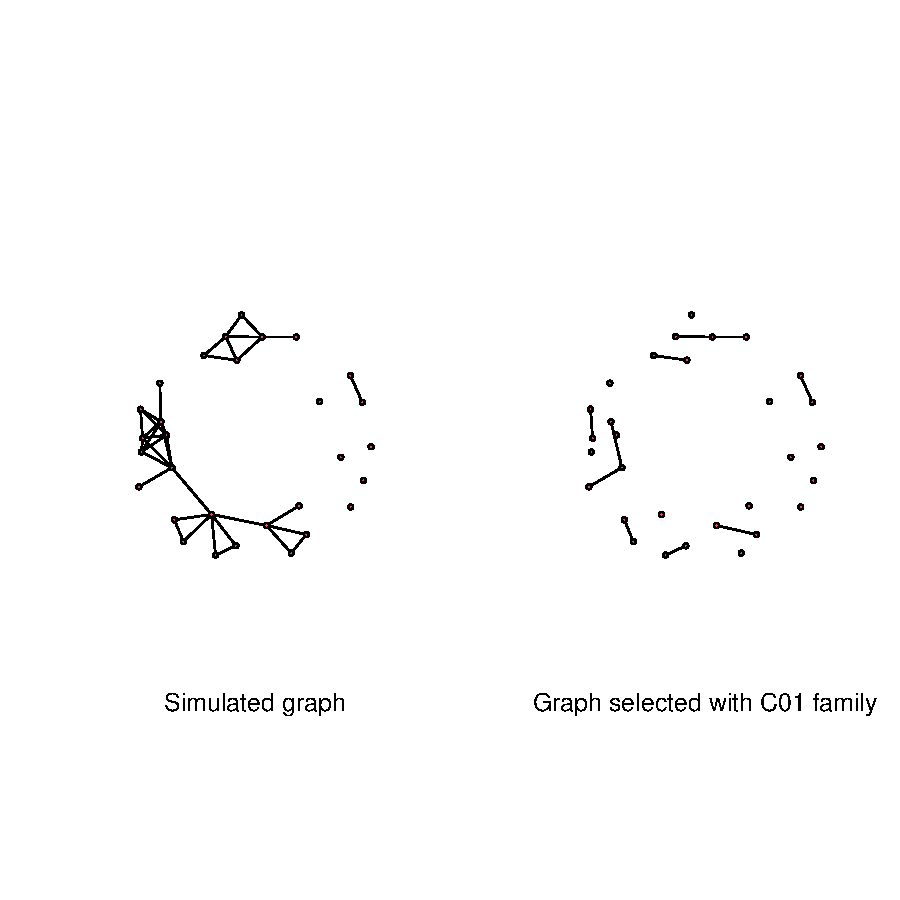
\includegraphics{Notice-explotFast}
\begin{Schunk}
\begin{Sinput}
> # ----------------------------------------
> # Graph selection with family QE:  use of selectQE
> # ----------------------------------------
> GQE <- selectQE(X)
> # ----------------------------------------
> # Plot the result
> # ----------------------------------------
> 
\end{Sinput}
\end{Schunk}
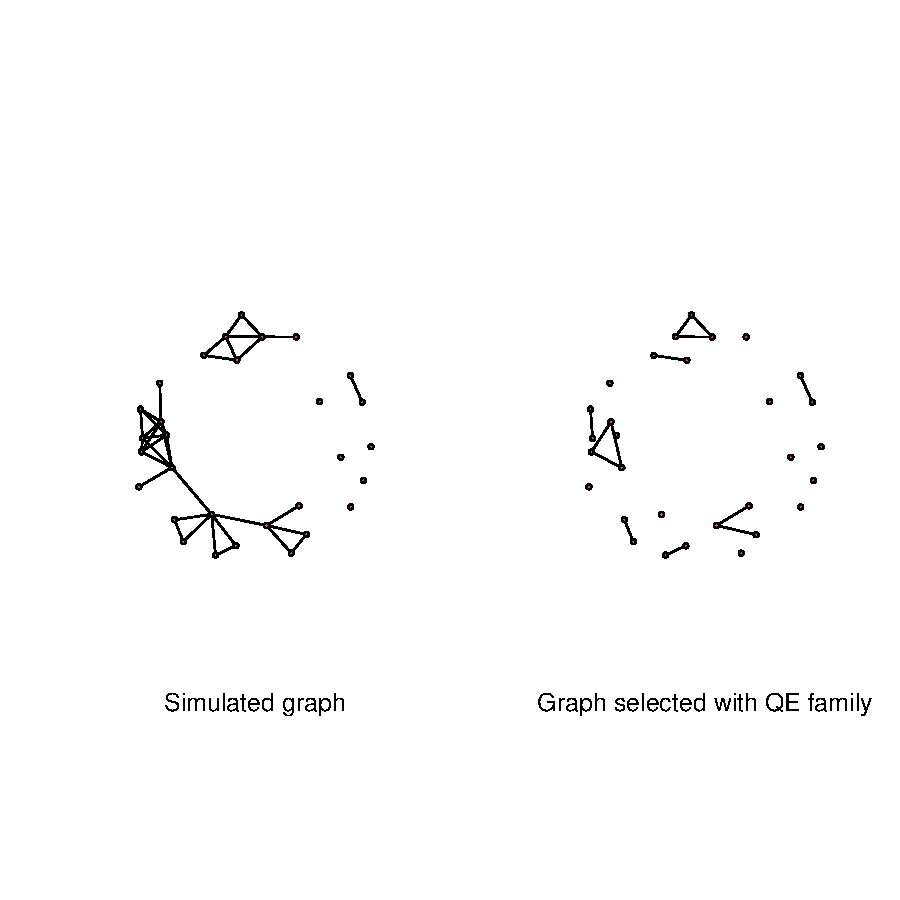
\includegraphics{Notice-explotQE}
\begin{Schunk}
\begin{Sinput}
> # ----------------------------------------
> # Graph selection with selectMyFam
> # ----------------------------------------
> # generate a family of candidate graphs with glasso
> library("glasso")
> MyFamily <- NULL
> for (j in 1:3){
+   MyFamily[[j]] <- abs(sign(glasso(cov(X),rho=j/5)$wi))
+   diag(MyFamily[[j]]) <- 0
+ }
> # select a graph within MyFamily
> GMF <- selectMyFam(X,MyFamily)
> # ----------------------------------------
> # Plot the result
> # ----------------------------------------
> 
> 
\end{Sinput}
\end{Schunk}
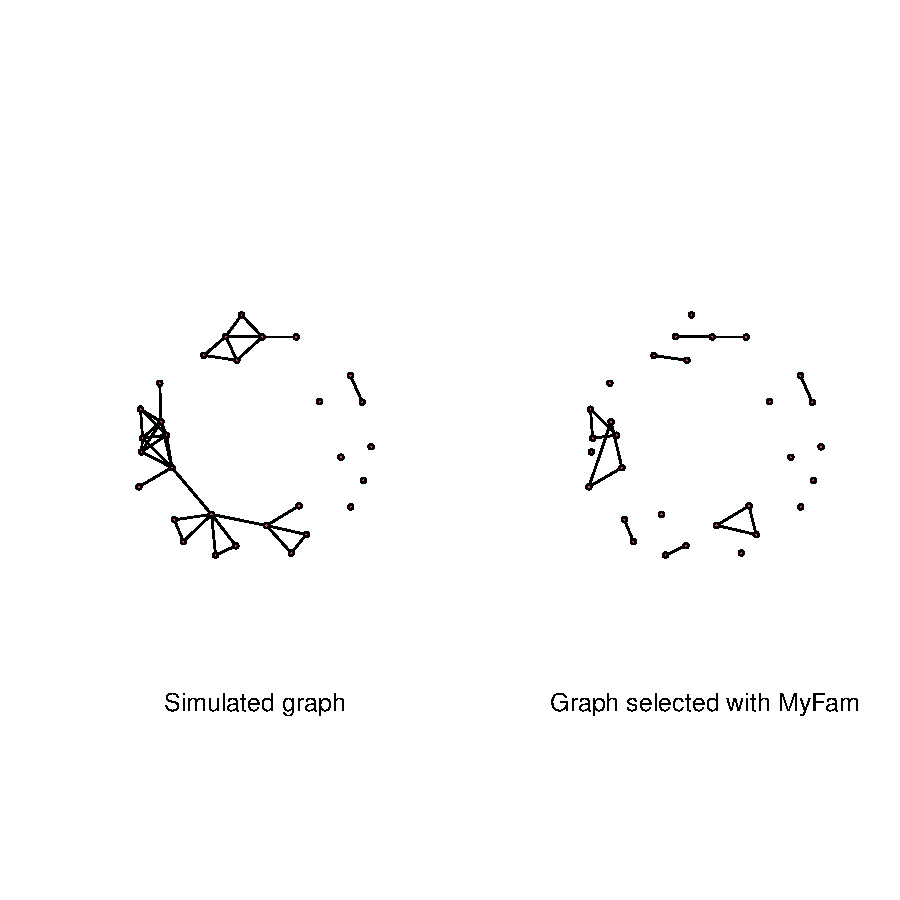
\includegraphics{Notice-explotMyFam}



%\addcontentsline{toc}{section}{References}

\bibliographystyle{abbrv}
%\bibliographystyle{acmtrans-ims}


\bibliography{estimation}

\end{document}
        
